% 9 variables in here:
% h_1 = 10.0, h_2 = 10.0, h_3 = 10.0, ux_1 = 0.0, ux_2 = 1.0, ux_3 = 1.0, uy_1 = 0.0, uy_2 = 1.0, uy_3 = 1.0
\begin{figure}[ht!]
\centering
  % \quad \subfloat[] {
  %   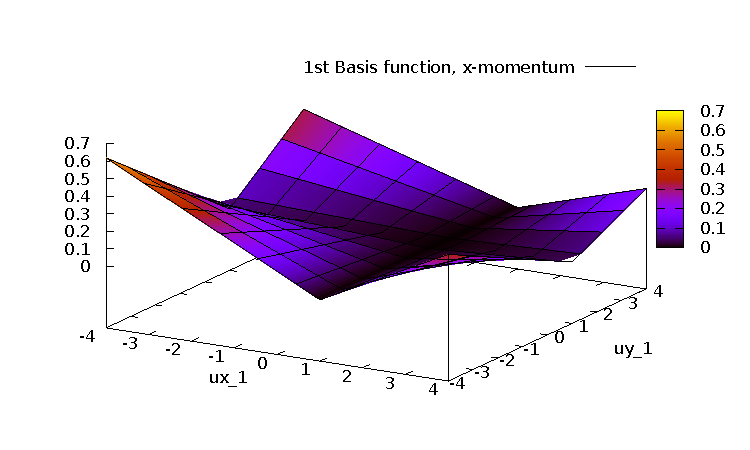
\includegraphics[scale=\zoomfactor]{{{ord1_varying_ux1_uy1_differing_ux2_uy2_ux3_uy3_1_1_1_1/10.0_10.0_10.0_x_1.0_1.0_y_1.0_1.0f0}}}
  % }
  \quad \subfloat[$SE_x^1$] {
    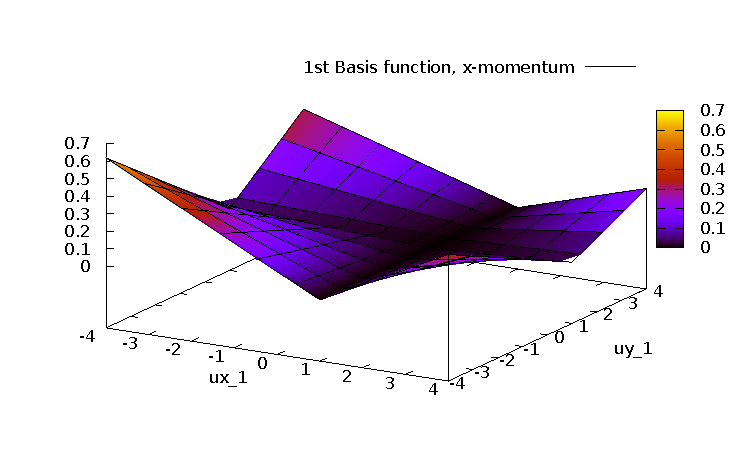
\includegraphics[scale=\zoomfactor]{{{ord1_varying_ux1_uy1_differing_ux2_uy2_ux3_uy3_1_1_1_1/10.0_10.0_10.0_x_1.0_1.0_y_1.0_1.0f00}}}
  }
  % \quad \subfloat[] {
  %   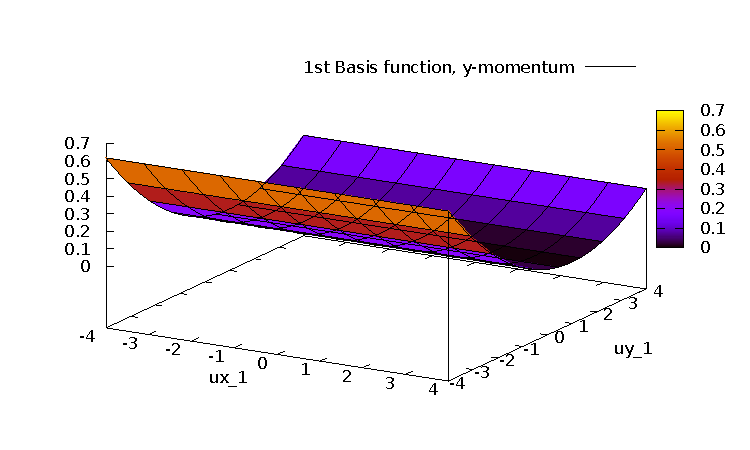
\includegraphics[scale=\zoomfactor]{{{ord1_varying_ux1_uy1_differing_ux2_uy2_ux3_uy3_1_1_1_1/10.0_10.0_10.0_x_1.0_1.0_y_1.0_1.0f01}}}
  % }
  \quad \subfloat[$SE_x^2$] {
    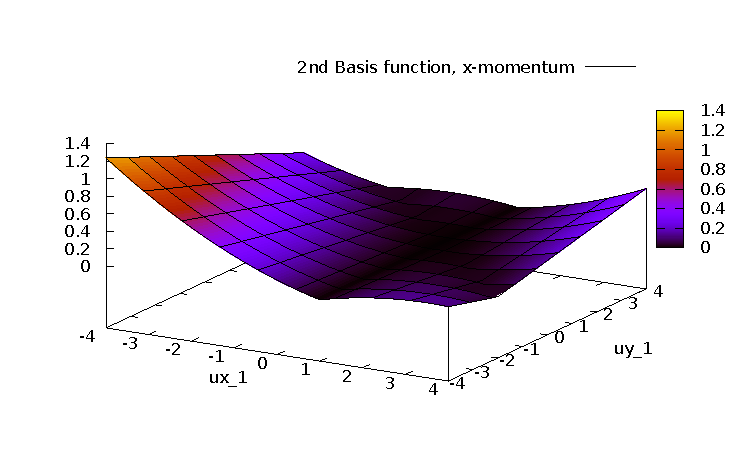
\includegraphics[scale=\zoomfactor]{{{ord1_varying_ux1_uy1_differing_ux2_uy2_ux3_uy3_1_1_1_1/10.0_10.0_10.0_x_1.0_1.0_y_1.0_1.0f02}}}
  }
  % \quad \subfloat[] {
  %   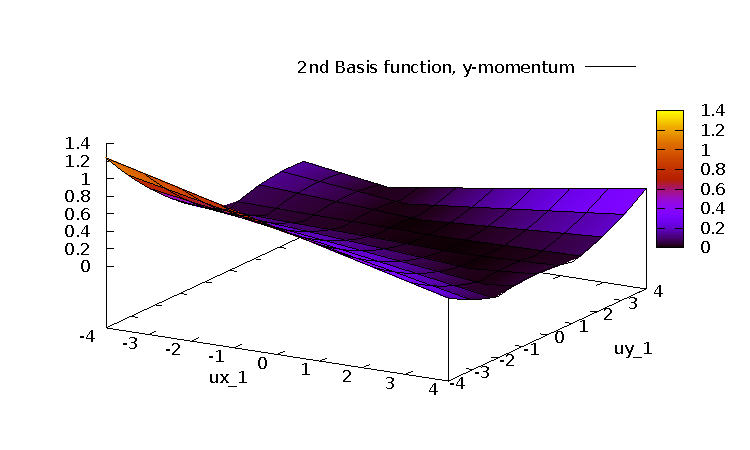
\includegraphics[scale=\zoomfactor]{{{ord1_varying_ux1_uy1_differing_ux2_uy2_ux3_uy3_1_1_1_1/10.0_10.0_10.0_x_1.0_1.0_y_1.0_1.0f03}}}
  % }
  \quad \subfloat[$SE_x^3$] {
    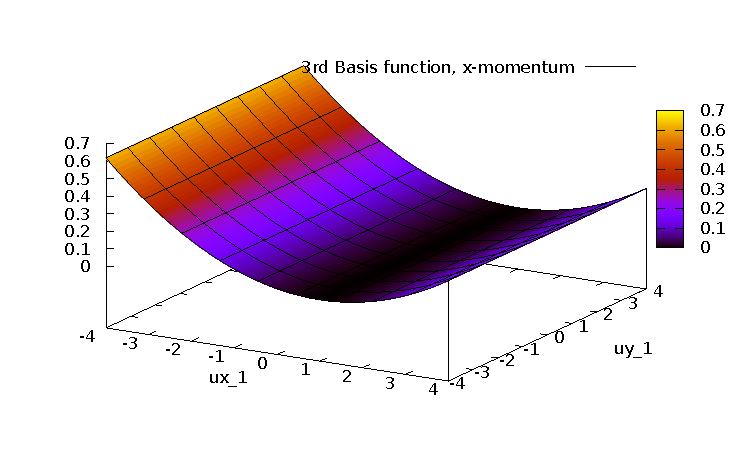
\includegraphics[scale=\zoomfactor]{{{ord1_varying_ux1_uy1_differing_ux2_uy2_ux3_uy3_1_1_1_1/10.0_10.0_10.0_x_1.0_1.0_y_1.0_1.0f04}}}
  }
  % \quad \subfloat[] {
  %   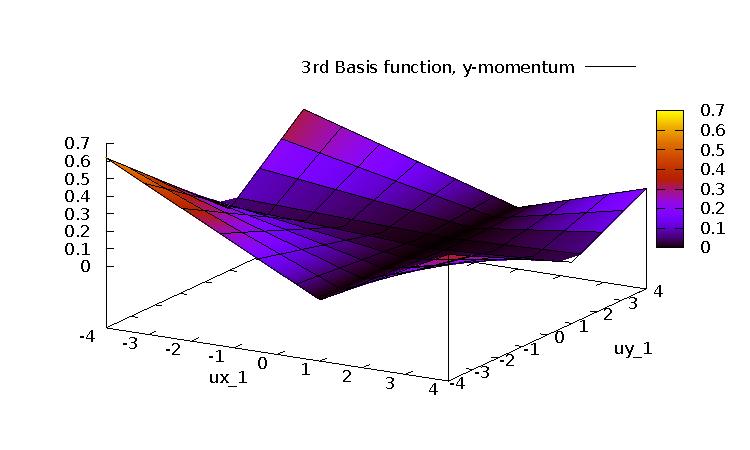
\includegraphics[scale=\zoomfactor]{{{ord1_varying_ux1_uy1_differing_ux2_uy2_ux3_uy3_1_1_1_1/10.0_10.0_10.0_x_1.0_1.0_y_1.0_1.0f05}}}
  % }
  % \quad \subfloat[] {
  %   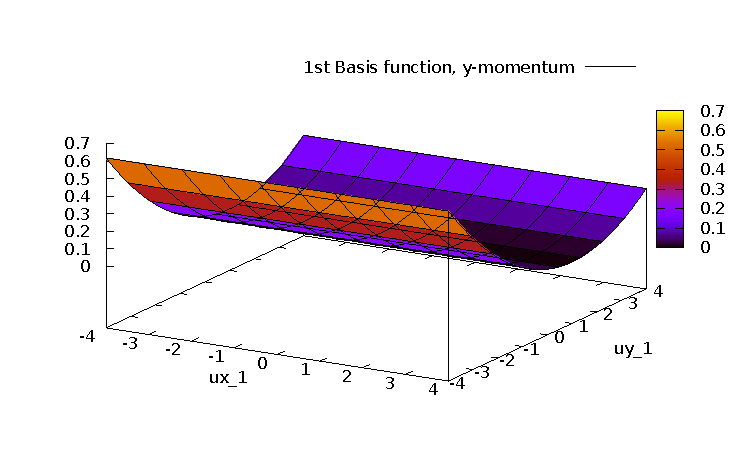
\includegraphics[scale=\zoomfactor]{{{ord1_varying_ux1_uy1_differing_ux2_uy2_ux3_uy3_1_1_1_1/10.0_10.0_10.0_x_1.0_1.0_y_1.0_1.0f1}}}
  % }
  % \quad \subfloat[] {
  %   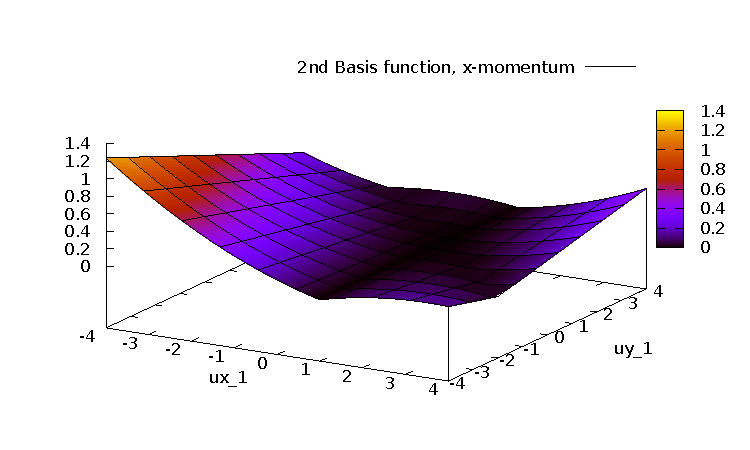
\includegraphics[scale=\zoomfactor]{{{ord1_varying_ux1_uy1_differing_ux2_uy2_ux3_uy3_1_1_1_1/10.0_10.0_10.0_x_1.0_1.0_y_1.0_1.0f2}}}
  % }
  % \quad \subfloat[] {
  %   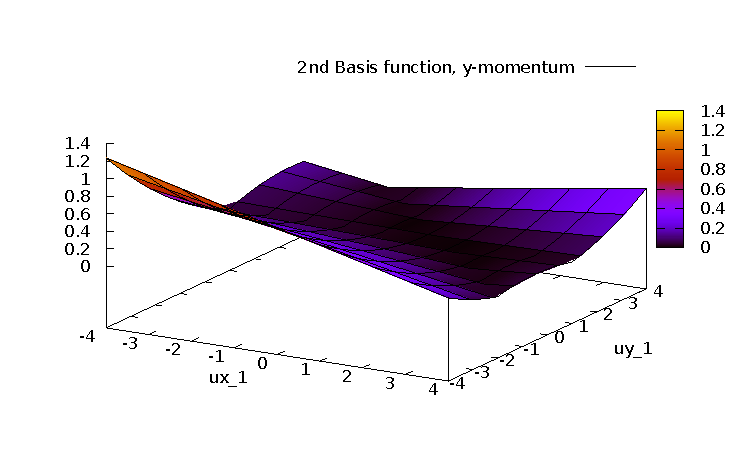
\includegraphics[scale=\zoomfactor]{{{ord1_varying_ux1_uy1_differing_ux2_uy2_ux3_uy3_1_1_1_1/10.0_10.0_10.0_x_1.0_1.0_y_1.0_1.0f3}}}
  % }
  % \quad \subfloat[] {
  %   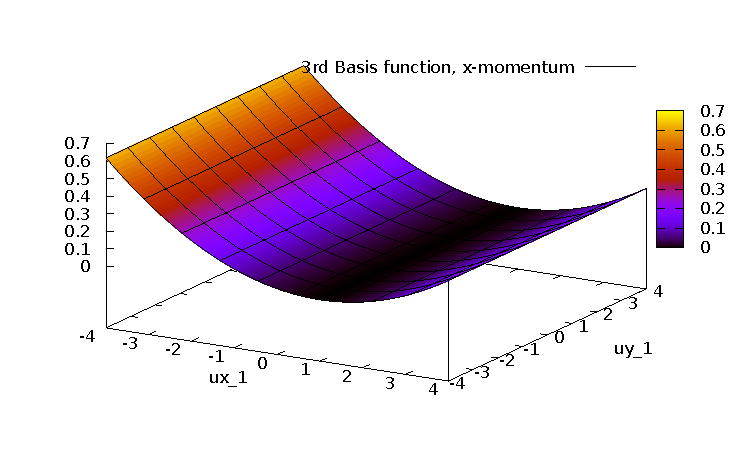
\includegraphics[scale=\zoomfactor]{{{ord1_varying_ux1_uy1_differing_ux2_uy2_ux3_uy3_1_1_1_1/10.0_10.0_10.0_x_1.0_1.0_y_1.0_1.0f4}}}
  % }
  % \quad \subfloat[] {
  %   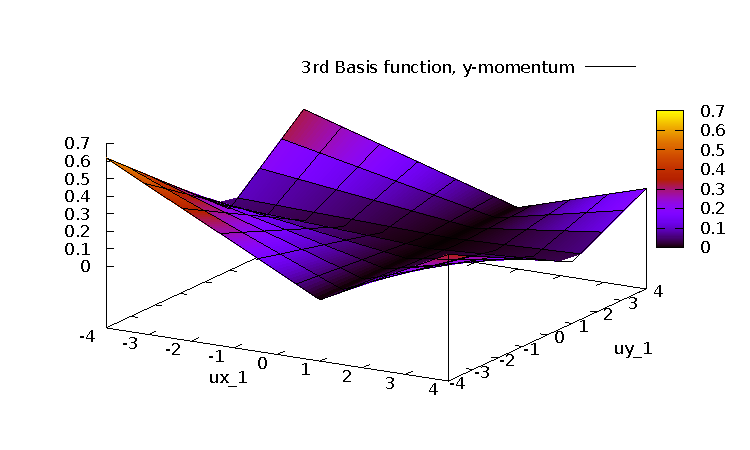
\includegraphics[scale=\zoomfactor]{{{ord1_varying_ux1_uy1_differing_ux2_uy2_ux3_uy3_1_1_1_1/10.0_10.0_10.0_x_1.0_1.0_y_1.0_1.0f5}}}
  % }
\caption{All height values are set to 10, $u_{x,2} = 1.0, u_{x,3} = 1.0, u_{y,2} = 1.0, u_{y,3} = 1.0$. Symmetry is as described in figure \ref{fig:ord1_varying_ux1_uy1_differing_ux2_uy2_3_3}.}
\label{fig:ord1_varying_ux1_uy1_differing_ux2_uy2_ux3_uy3_1_1_1_1}
\end{figure}

%%% Local Variables:
%%% TeX-master: "../results.tex"
%%% End:
